\chapter{Proposed method}


The main objective of this thesis is to carry out a comprehensive comparison of various methods for time series classification, specifically those that deal with missing data.
To achieve this goal, we implemented multiple machine learning models to evaluate their efficacy on a comprehensive dataset of Satellite Image Time Series.
The comparison and evaluation of these models will help in determining the most effective approach to handle missing data and enhance the accuracy of time series classification tasks.


\section{Data preparation}

In order to ensure a comprehensive and unbiased comparison, the same dataset and evaluation metrics were employed for all machine learning models in this thesis. 
Specifically, the dataset of choice was the Satellite Image Time Series (SITS) dataset, which comprises a total of 137,606 time series of satellite images covering natural and semi-natural areas. 
As the available data for this task is relatively limited, k-fold cross validation with $k=5$ and varying seeds was implemented to guarantee that the results were not influenced by the partitioning of the dataset. Additionally, to ensure a balanced distribution of classes within each fold, the dataset was split into training/validation/test sets with equal representation of each class. 
To prevent spatial correlation, the same polygon pixels were not placed in the same sets.

The distribution of polygons and pixels for each class in the training, validation, and test sets can be observed in Table \ref{tab:dataset-splits}.
The split was conducted in a ratio of 60:20:20 for the training, validation, and test sets respectively, and no spatial correlation was taken into account during the partitioning process.
The table provides a comprehensive summary of the number of polygons and pixels for each class in each of the sets.

\begin{table}[H]
  \begin{tabular}{crrlcrrlcrrl}
     \cline{2-4} \cline{6-8} \cline{10-12} \\[-0.2cm]
          & \multicolumn{3}{c}{Train}                                 & \multicolumn{1}{l}{} & \multicolumn{3}{c}{Validation}                            & \multicolumn{1}{c}{} & \multicolumn{3}{c}{Test} \\[0.1cm]
    Class & Pol.                    & Pix.                      & \%  &                      & Pol.                    & Pix.  & \%                      &                      & Pol.   & Pix.    & \%    \\[0.2cm] \cline{2-4} \cline{6-8} \cline{10-12} \\[-0.2cm]
    1     & 427                     & 6486                      & 7   &                      & 142                     & 2266  & 8                       &                      & 143    & 1660    & 6     \\
    2     & 196                     & 3369                      & 3   &                      & 65                      & 803   & 3                       &                      & 67     & 993     & 3     \\
    3     & 49                      & 21298                     & 24  &                      & 16                      & 5308  & 20                      &                      & 17     & 5489    & 21    \\
    4     & 103                     & 30631                     & 35  &                      & 34                      & 8194  & 31                      &                      & 35     & 10350   & 40    \\
    5     & 133                     & 16933                     & 19  &                      & 44                      & 6362  & 24                      &                      & 46     & 5372    & 20    \\
    6     & 19                      & 1428                      & 1   &                      & 6                       & 309   & 1                       &                      & 7      & 338     & 1     \\
    7     & 23                      & 3399                      & 3   &                      & 7                       & 948   & 3                       &                      & 9      & 858     & 3     \\
    8     & 33                      & 2595                      & 3   &                      & 11                      & 1455  & 5                       &                      & 12     & 762     & 2     \\[0.2cm]\hline \\[-0.2cm]
    Tot   & \multicolumn{1}{l}{983} & \multicolumn{1}{l}{86139} & 100 & \multicolumn{1}{l}{} & \multicolumn{1}{l}{325} & 25645 & \multicolumn{1}{l}{100} & \multicolumn{1}{l}{} & 336    & 25822   & 100       
  \end{tabular}
  \caption{Distribution of classes, polygons and pixels for each dataset.}
  \label{tab:dataset-splits}
\end{table}

\section{Models}
To start the process of selecting the most promising models for time series classification, the research began by conducting an extensive review of the current state of the art in the field. This involved a thorough investigation of published research studies and academic papers that were relevant to the research question. 
After analyzing and comparing the different approaches presented in the literature, the most promising models were selected to be further explored and tested.

Following the model selection phase, the research continued by studying the papers in-depth and examining any available source code.
This process allowed us to gain a better understanding of the underlying algorithms and techniques used in each model, as well as any implementation details that may be relevant for adaptation to the specific research needs.
Once the code was examined, it was adapted or implemented to suit our requirements, and the performance of each model was evaluated on our dataset.

Except for the transformer models, which have been implemented using PyTorch \cite{NEURIPS2019_9015}, all the other models in this study have been implemented using TensorFlow \cite{tensorflow2015-whitepaper}.
TensorFlow is a popular and widely used open-source machine learning framework developed by Google, which provides an efficient and flexible way to build and train neural networks.
On the other hand, PyTorch is another popular open-source machine learning framework developed by Facebook, which provides dynamic computational graphs and a more pythonic way to build and train neural networks, making it particularly suitable for research purposes.

Using both TensorFlow and PyTorch for implementing the models was a challenging task, but it provided an opportunity to improve my skills in working with different deep learning frameworks.

In order to optimize the performance of each model, we conducted a thorough exploration of the hyperparameter space, varying different parameters such as learning rate, batch size, number of layers, number of units per layer, activation functions, regularization techniques, and others.
Additionally, based on the findings reported by the authors of each model, we also experimented with modifications to the architecture of the network, such as the addition of new layers, changing the sequence of layers, or adjusting the size of the filters in convolutional layers.

This process of hyperparameter tuning and model modification allowed us to identify the optimal settings for each model on our specific dataset, resulting in the best possible performance in terms of accuracy.
It is worth noting that this process was not always straightforward, and in some cases, we encountered challenges such as overfitting, convergence issues, or long training times.
Nevertheless, we were able to overcome these obstacles through careful experimentation and iteration.

During our experiments, we explored various methods to handle missing data in time series classification. 
In order to fully understand the impact of missing values on the performance of our models, we implemented two different approaches.
The first method involved replacing the missing values with zeros, while the second method involved using pre-imputed values based on linear multi-temporal interpolation \cite{IENCO201911}, which utilized the available cloud masks to fill the gaps in the time series data. 
By implementing both methods, we were able to compare the performance of the models in handling missing data in different ways.


\section{Weights and Biases}
% TODO: talk about wandb

In order to keep track of the experiments, we used Weights and Biases\cite{wandb} (wandb) to log the configuration and the results of the experiments.
This was very useful to compare the results of the different models. It also helped to keep the models reproducible and to fine-tune the hyperparameters of the models.

\begin{figure}[H]
  \centering
  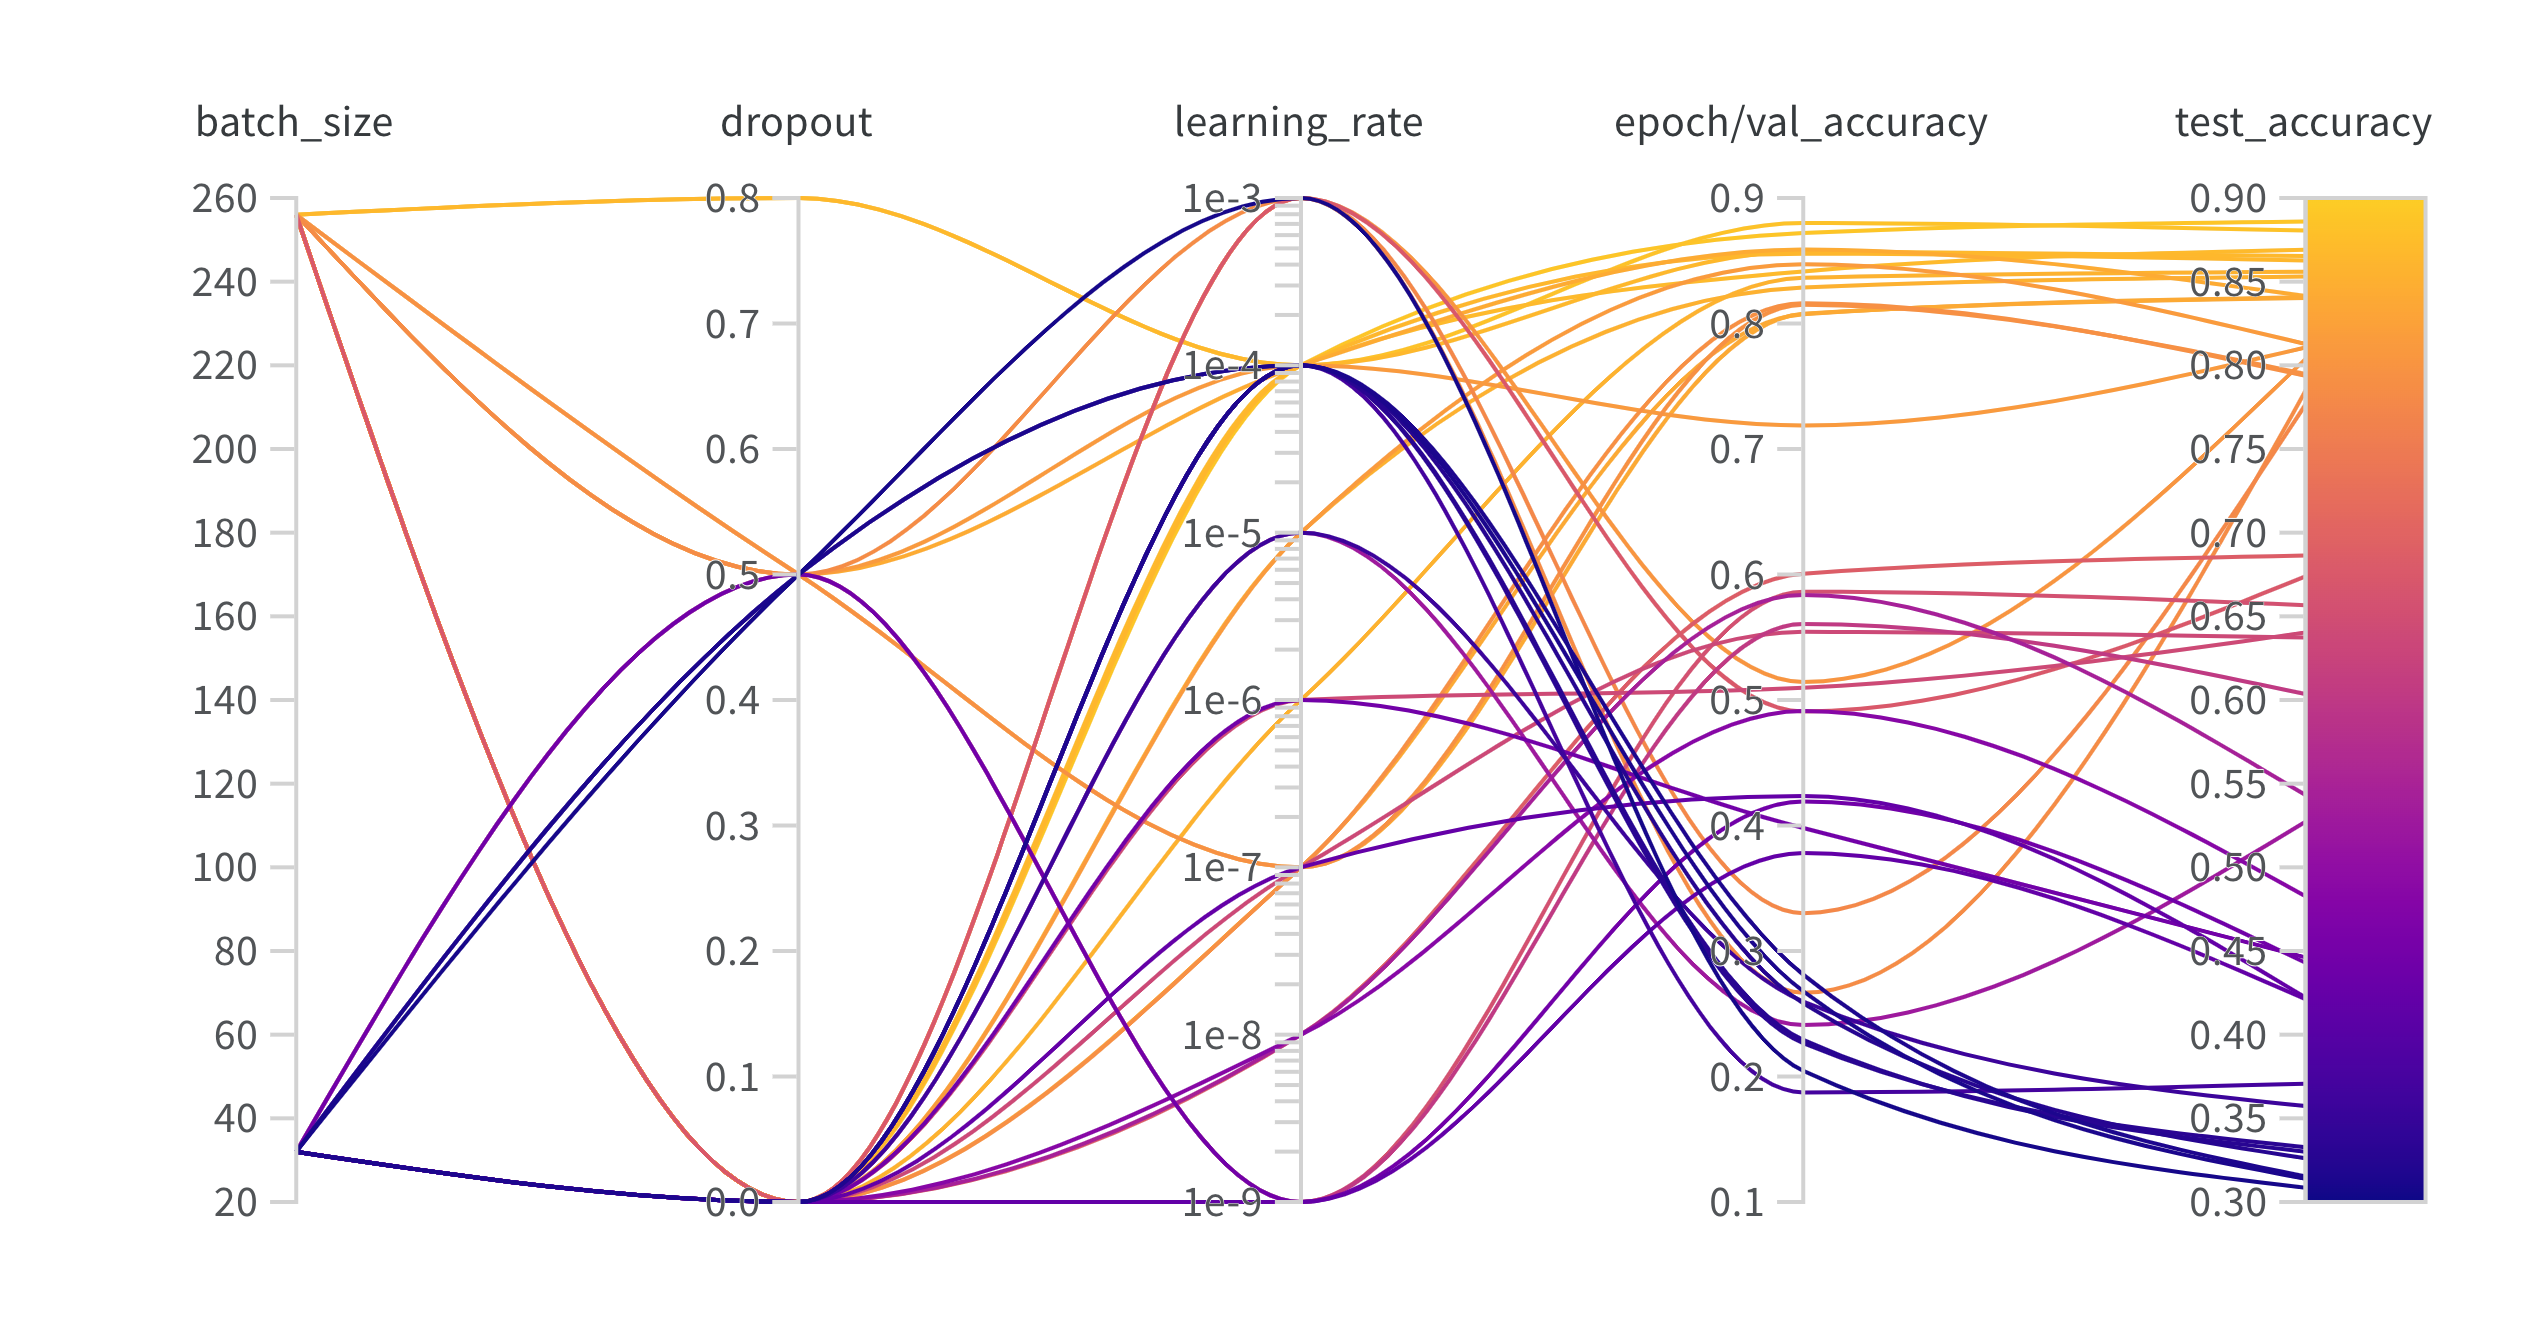
\includegraphics[width=0.9\textwidth]{wandb1}
  \caption{Example of parallel coordinates plot in wandb}
\end{figure}

\begin{figure}[H]
  \centering
  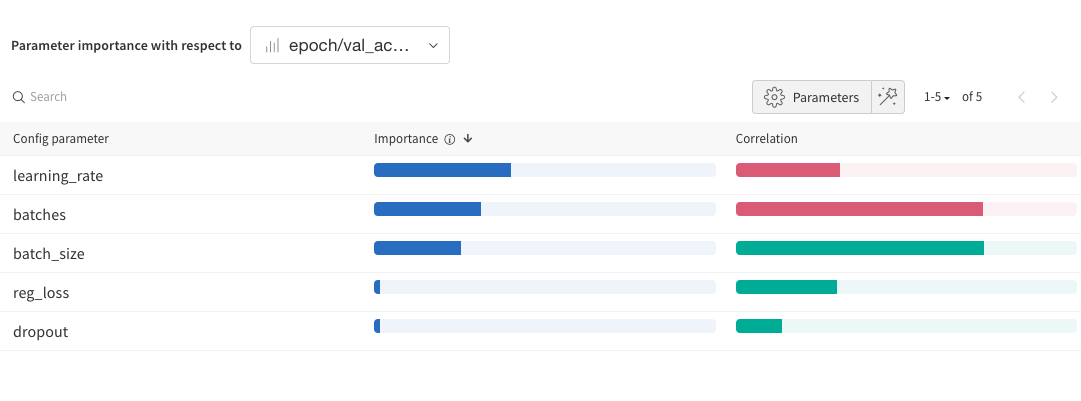
\includegraphics[width=0.9\textwidth]{wandb2}
  \caption{Example of Parameter importance panel in wandb}
\end{figure}




